\section{Достоверность партонной модели при ПэВ-энергиях}
\subsection{Области фазового пространства $(x, Q^2)$}
Как упоминалось ранее, дважды-дифференциальные сечения являются функциями энергии нейтрино $E_{\nu}$ и Бьеркеновских переменных $x$ и $y$. Но также можно описывать сечение в переменных $(E_{\nu}, x,Q^2)$, где $Q^2 = 2M_NExy$ - квадрат переданного 4-импульса лептона нуклону. Переменная Бъеркена $x$ изменяется от 0 до 1. Переменная $Q^2$ для ГНР (для рассмотренных партонных моделей) имеет минимальное значение порядка $1$ $\text{ГэВ}^2$. На рис. (\ref{RD}) можно видеть реальные данные \cite{ParticleDataGroup:2024cfk}, полученные в экспериментах на коллайдерах и в экспериментах с фиксированной мишенью.  
\begin{figure}[!h]
\centering
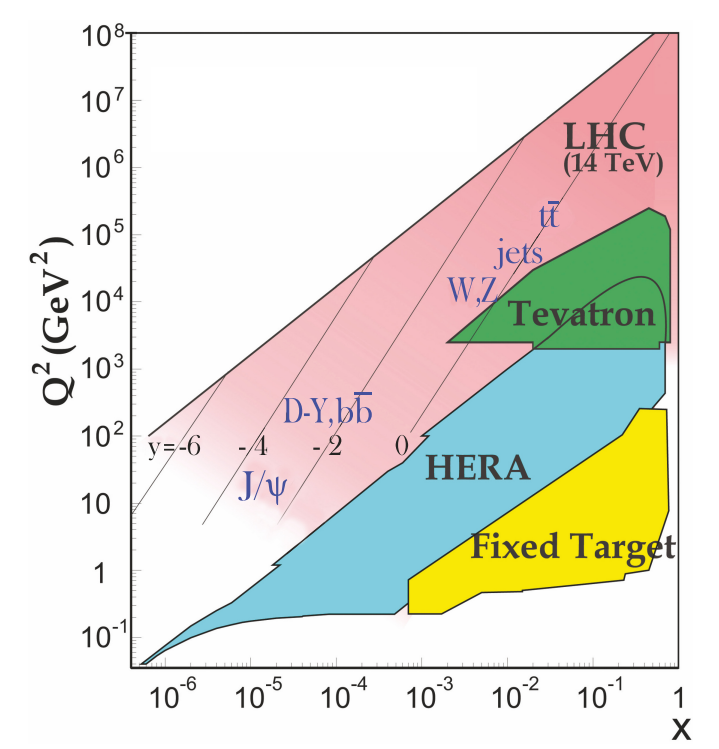
\includegraphics[width=\linewidth]{images/NuProp/reald}
\caption{Кинематические области в $x$ и $Q^2$, исследованные в экспериментах с неподвижной мишенью и на коллайдере \cite{ParticleDataGroup:2024cfk}.}
\label{RD}
\end{figure}
\subsection{Визуализация 2D-сечений с отсечками}
Можно поглядеть, как сечения, получаемые с помощью nudisxs, связаны с экспериментальными данными. На графиках (\ref{Pp3})-(\ref{Pp8}) можно увидеть зависимость кумулятивного нормированного сечения $F_{\sigma}(x,Q^2)$, которое определено следующим образом: 
 \begin{equation}
     F_{\sigma}(x,Q^2) = \frac{1}{\sigma(E_{\nu})}\int\limits_{x}^1dx\int\limits_{Q^2}^{Q^2_{max}}dQ^2\frac{d^2\sigma}{dxdQ^2}.
 \end{equation}
 Здесь $\frac{d^2\sigma}{dxdQ^2}$ - дважды-дифференциальное сечение рассеяния нейтрино на нуклоне. Линии указывают области, где сечения насыщаются до определенного уровня. Серая штриховка показываетэкспериментально доступную область. Видно, что область насыщения сечений частично выходит из области экспериментальных данных. При высоких энергиях  - это область в диапазоне $10^2\le Q^2\le10^{4.5} $ и $10^{-5}\le x \le 10^{-9}$.  
 \begin{figure}[!h]
\centering
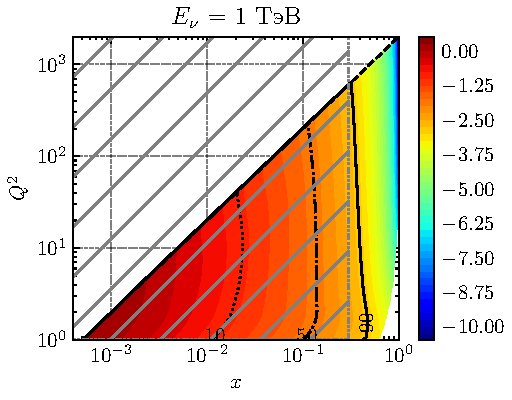
\includegraphics[width=0.97\linewidth]{images/NuProp/cdfxq2_cc_proton_CT18ZNNLO_14_1000.pdf}
\caption{Зависимость кумулятивного нормированного сечения $F_{\sigma}(x,Q^2)$ в зависимости от переменной Бъеркена $x$ и переменной $Q^2$ для энергии нейтрино $E_{\nu} = 1$ TeV для модели партонных распределений CTEQ15\cite{ncteq15}. }
\label{Pp3}
\end{figure}
\begin{figure}[!h]
\centering
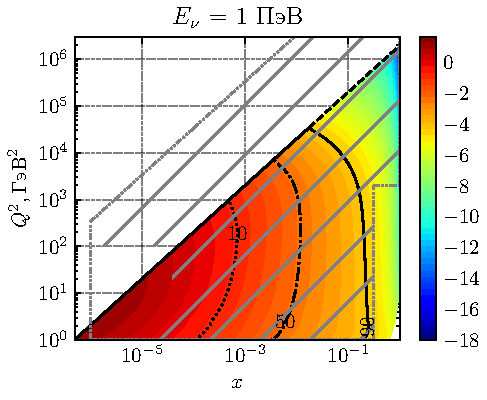
\includegraphics[width=0.97\linewidth]{images/NuProp/cdfxq2_cc_proton_CT18ZNNLO_14_1000000.pdf}
\caption{Зависимость кумулятивного нормированного сечения $F_{\sigma}(x,Q^2)$ в зависимости от переменной Бъеркена $x$ и переменной $Q^2$ для энергии нейтрино $E_{\nu} = 1$ PeV для модели партонных распределений CTEQ15\cite{ncteq15}.}
\label{Pp6}
\end{figure}
\begin{figure}[!h]
\centering
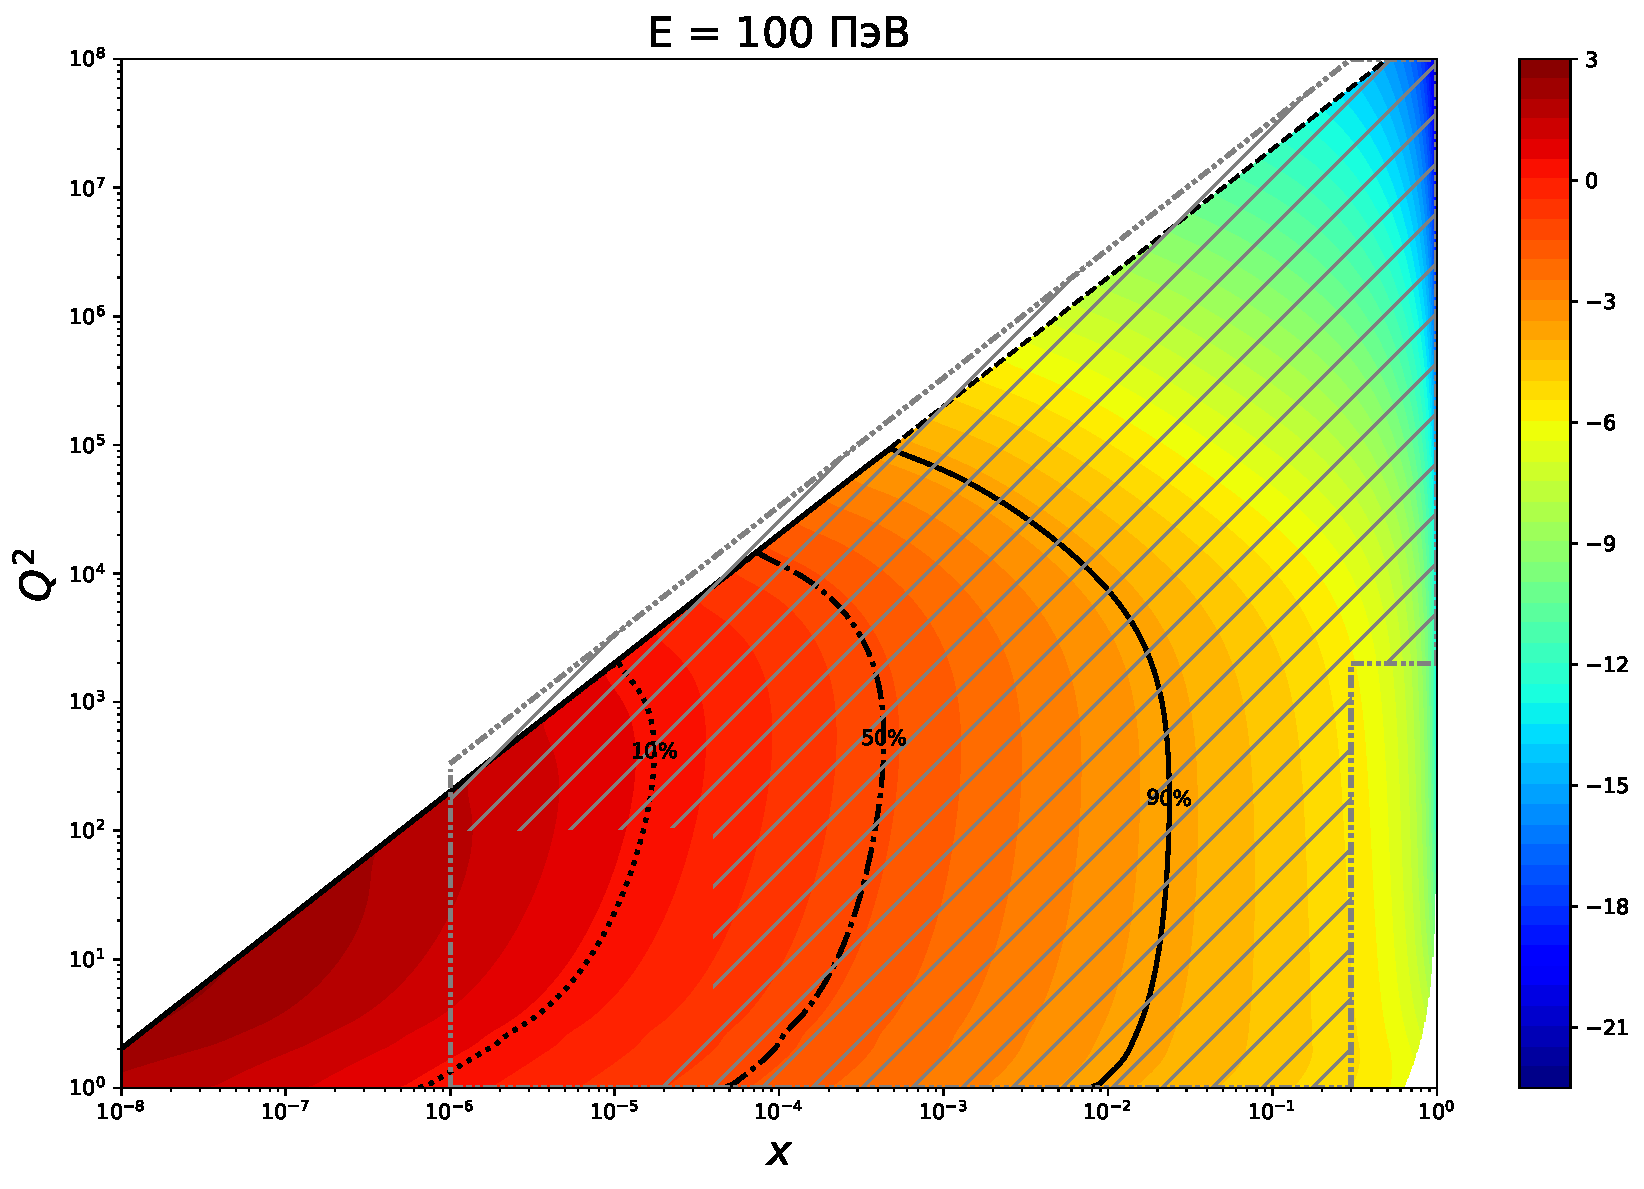
\includegraphics[width=0.97\linewidth]{images/NuProp/cdfxq2_cc_proton_CT18ZNNLO_14_100000000.pdf}
\caption{Зависимость кумулятивного нормированного сечения $F_{\sigma}(x,Q^2)$ в зависимости от переменной Бъеркена $x$ и переменной $Q^2$ для энергии нейтрино $E_{\nu} = 100$ PeV для модели партонных распределений CTEQ15\cite{ncteq15}.}
\label{Pp8}
\end{figure}
